\documentclass[10pt]{article}

\usepackage[table]{xcolor}
\usepackage{mathrsfs} % for mathscr
\usepackage{amssymb,amsmath}
\usepackage{graphicx}
\usepackage{hyperref} 
\usepackage{multirow}
%\usepackage{scrextend}
\usepackage{xspace}
\usepackage{booktabs}
%\usepackage{enumitem} 
\usepackage{caption} 
\usepackage{subcaption} 
\usepackage{comment}
\usepackage{longtable}
%\usepackage{subfigure}

% tuning toc, chapters, list items
\hypersetup{colorlinks,linkcolor={red!50!black},citecolor={blue!50!black},urlcolor={blue!80!black}}
\usepackage[toc,page]{appendix}
\usepackage[top=1.5in, bottom=1.5in, left=1.41in, right=1.41in]{geometry}
%\usepackage{titlesec}
%\newcommand{\chapnumfont}{\usefont{T1}{pnc}{b}{n}\fontsize{100}{100}\selectfont}
%\colorlet{chapnumcol}{gray!75}  % color for chapter number
%\titleformat{\chapter}[display]{\filleft\bfseries}{\filleft\chapnumfont\textcolor{chapnumcol}{\thechapter}}{-24pt}{\Huge}
%\setlist{topsep=2.2pt,itemsep=0.5pt} %nolistsep}%\setlist[itemize]{itemsep=0.5pt}

\usepackage{tikz}
\usetikzlibrary{shapes,calc,positioning,automata,arrows,trees}
\usepackage[tikz]{bclogo}
\renewcommand\logowidth{15pt}
\newcommand\bcpenr{\includegraphics[width=\logowidth]{crayonRed.png}} 
\newcommand\bcpen{\includegraphics[width=\logowidth]{figures/crayonBlue.png}} 
\newcommand\bcdico{\includegraphics[width=\logowidth]{figures/bookJaune.png}} 
\newcommand\bcroue{\includegraphics[width=\logowidth]{figures/roue.png}} 
%\renewcommand\bcStyleTitre[1]{\large\textbf{#1}}
%\usepackage[skins,breakable,xparse]{tcolorbox}

\newcounter{cntM3}
\newcounter{cntSy}
\newcounter{cntSe}
\newcounter{cntEx}

\usepackage{listingsutf8}

\newtheorem{definition}{Definition}
\newtheorem{remark}{Remark}
\newtheorem{remarks}{Remarks}

\definecolor{v3lgray}{gray}{0.98}
\definecolor{v2lgray}{gray}{0.85}
\definecolor{vlgray}{gray}{0.92}
\definecolor{mygray}{rgb}{0.92,0.98,0.92}
\definecolor{bgray}{rgb}{0.8,0.8,0.8}
\definecolor{dgray}{rgb}{0.4,0.4,0.4}
\definecolor{dblue}{RGB}{0,0,99}
\definecolor{dred}{RGB}{150,6,54}
\definecolor{dgreen}{RGB}{47,135,7}
\definecolor{d2green}{RGB}{47,85,7}
\definecolor{dviolet}{RGB}{102,0,153}
\definecolor{mblue}{RGB}{0,0,180}
\definecolor{m2blue}{RGB}{0,0,220}
\definecolor{colorse}{RGB}{255,248,220}
\definecolor{colorsy}{HTML}{F2F2F2}
\definecolor{colorex}{HTML}{FFE3BE}
\definecolor{grey}{rgb}{0.75,0.75,0.75}
\definecolor{dgray}{rgb}{0.4,0.4,0.4}

\def\N{\mathbb{N}}
\def\Q{\mathbb{Q}}
\def\D{{\mathsf{D}}}
\def\B{{\mathsf{B}}}
\def\DINT{{\mathsf{D}_\mathsf{int}}}
\def\BINT{{\mathsf B}_\mathsf{int}} 
\def\ti{\textrm{-}}
\def\tr{\;\!\triangleright}
\def\st{\!:\!}

\def\gecode{Gecode\xspace}
\def\choco{Choco3\xspace}
\def\abscon{AbsCon\xspace}
\def\mzinc{MiniZinc\xspace}
\def\jacop{JaCoP\xspace}
\def\minion{Minion\xspace}
\def\xt{{\rm XCSP3}\xspace}
\def\cat{Global Constraint Catalog\xspace}

\newcommand{\xml}[1]{{\tt <#1>}} % xml element names
\newcommand{\att}[1]{{\tt #1}} % attribute names
\newcommand{\val}[1]{{\tt "#1"}} % attribute values

\newcommand{\bnf}[1]{\textsl{\color{dblue}{#1}}}
\newcommand{\bnfX}[1]{\texttt{<}\bnf{#1}\texttt{.../>}}
\newcommand{\norX}[1]{\texttt{<#1.../>}}

%\newcommand{\gb}[1]{\textcolor{dgreen}{{\tt #1}}} % global constraint names
\newcommand{\gb}[1]{{\tt #1}} % global constraint names
\newcommand{\gbc}[1]{\textcolor{dblue}{{\mathit #1}}} % global constraint names
\newcommand{\nn}[1]{{\tt #1}} % name normal
\newcommand{\nm}[1]{\mathit{#1}} % name math
\newcommand{\sy}[1]{{\ttfamily {\slshape #1}}}  % syntax elements like intValue etc.
\newcommand{\ns}[1]{{\mathcal #1}}  % symbol for set variables
\newcommand{\nss}[1]{{\mathbfcal #1}}  % symbol for set variables


\newcommand{\violet}[1]{{\small \textcolor{dviolet}{#1}}}

\newcommand{\va}[1]{{\boldsymbol #1}} % value of variable (for semantics)
%\newcommand{\va}[1]{\underline{#1}} % value of variable (for semantics)
%\newcommand{\va}[1]{#1} % value of variable (for semantics)

%\newcommand{\todoguys}[1]{\fbox{{\textcolor{red}{{\bf TODO : #1}}}}}

%\usepackage{titlesec}
%\setcounter{secnumdepth}{4}
%\setcounter{tocdepth}{3} 

\def\mt{{\rm MCSP3}\xspace}
\def\xt{{\rm XCSP3}\xspace}


\lstset{
language=Java,
basicstyle=\small, %normalsize, % ou ça==> basicstyle=\scriptsize,
upquote=true,
aboveskip={\baselineskip},
columns=fullflexible,
showstringspaces=false,
extendedchars=true,
escapechar=ç,
breaklines=true,
showtabs=false,
showspaces=false,
showstringspaces=false,
identifierstyle=\ttfamily,
%keywordstyle=\color[rgb]{0,0,1},
commentstyle=\color[rgb]{0.133,0.545,0.133},
stringstyle=\color[rgb]{0.627,0.126,0.941},
backgroundcolor = \color{v3lgray},
}
\newcommand*{\com}[1]{\hfill \textcolor{dgray}{// #1}} % comment in lstlisting

\usepackage{verbatim}
\newenvironment{myvb}{\endgraf\small\verbatim}{\endverbatim}

\def\bef{\rule{10cm}{0.1mm}} %\medskip}
\def\aft{\rule{10cm}{0.1mm}\medskip}

\newcommand{\f}[1]{\mathtt{#1}} % for fields


\title{\textcolor{dred}{\mt \\ Easy Modeling for Everybody}\\ \textcolor{dred}{{\large Version 1.1}}}
\author{Christophe Lecoutre \\
CRIL CNRS, UMR 8188\\ University of Artois, France \\
%\\ Rue de l'universit\'e, SP 16\\ 62307 Lens, France \\
lecoutre@cril.fr
}

\date{December 17, 2018} %\\~ \\\href{www.xcsp.org}{www.xcsp.org}}


\begin{document}
\maketitle

\section{Introduction}

We propose a complete chain of production for solving combinatorial constrained problems. The two main ingredients are:
\begin{itemize}
\item MCSP3: a Java-based API for modeling constrained problems in a natural and declarative way
\item XCSP3: an intermediate format used to represent problem instances while preserving structure
\end{itemize}

\noindent A shown on the left of Figure \ref{fig:mcsp3}, the user has to:
\begin{itemize}
\item write a model using the Java modeling API called MCSP3
\item provide the data (in JSON format) for some specific instances
\item compile model and data in order to get XCSP3 files
\item solve the XCSP3 instance(s) using solvers like for example Choco or OscaR
\end{itemize}

\begin{figure}[p]
\begin{center}
\includegraphics[scale=0.2]{figures/user.png}
\smallskip

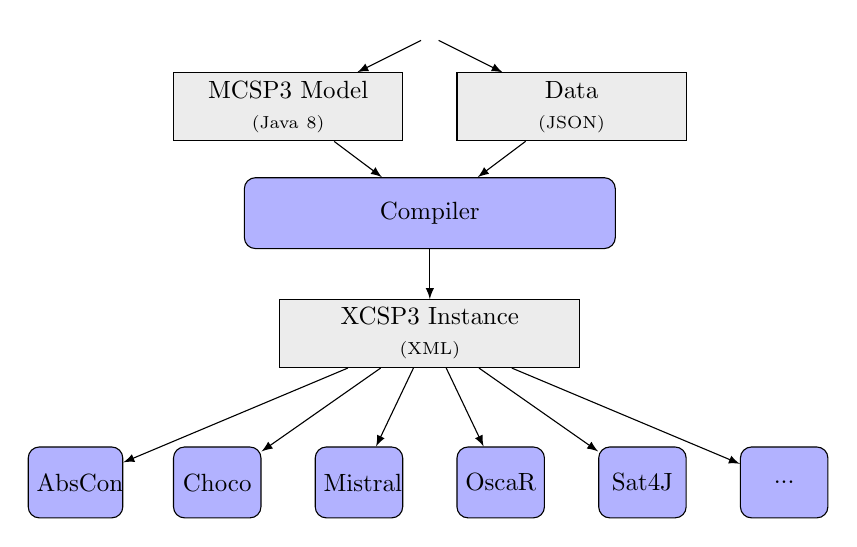
\begin{tikzpicture}[scale=0.9, every node/.style={scale=0.9}]
\tikzstyle{sn}=[draw,rounded corners,minimum height=10mm,fill=blue!30,text width=5cm,text centered]
%\node[draw=none,text centered,text width=2.3cm] (1) at (0,0) {Modeling}; 
%\node[draw=none,text centered,text width=2.3cm] (2) at (0,-2.5) {Intermediate\\ Format}; 
%\node[draw=none,text centered,text width=2.3cm] (2) at (0,-5) {Solvers}; 
\node[draw=none] (root) at (5,1.5) {};
\node[draw=none] (l) at (0,-1.25) {};
\node[draw=none] (r) at (9.5,-1.25) {};
\node[draw=none] (l2) at (0,-3.75) {};
\node[draw=none] (r2) at (9.5,-3.75) {};
%\node[draw=none] (a1) at (10,0.5) {$+$};
%\node[draw=none] (a2) at (10,-5.5) {$-$};
\node[draw,minimum height=7mm,fill=grey!30,text width=3cm,text centered] (model) at (3,0.5) {MCSP3 Model \\{\scriptsize (Java 8)}}; 
\node[draw,minimum height=7mm,fill=grey!30,text width=3cm,text centered] (data) at (7,0.5) {Data \\{\scriptsize (JSON)}}; 

\node[sn] (a) at (5,-1) {Compiler}; 
\node[draw,minimum height=7mm,fill=grey!30,text width=4cm,text centered] (b) at (5,-2.7) {XCSP3 Instance \\{\scriptsize (XML)}}; 
\node[sn,text width=1.1cm] (s1) at (0,-4.8) {AbsCon}; 
\node[sn,text width=1cm] (s2) at (2,-4.8) {Choco}; 
\node[sn,text width=1cm] (s3) at (4,-4.8) {Mistral};
\node[sn,text width=1cm] (s4) at (6,-4.8) {OscaR}; 
\node[sn,text width=1cm] (s5) at (8,-4.8) {Sat4J};
\node[sn,text width=1cm] (s6) at (10,-4.8) {...};
%\node[sn] (c) at (5,-5) {OscaR}; 
%\node[sn] (c) at (5,-5) {Sat4J}; 

\draw[->,>=latex] (root) -- (model);
\draw[->,>=latex] (root) -- (data);
\draw[->,>=latex] (model) -- (a);
\draw[->,>=latex] (data) -- (a);
\draw[->,>=latex] (a) -- (b);

\draw[->,>=latex] (b) -- (s1);
\draw[->,>=latex] (b) -- (s2);
\draw[->,>=latex] (b) -- (s3);
\draw[->,>=latex] (b) -- (s4);
\draw[->,>=latex] (b) -- (s5);
\draw[->,>=latex] (b) -- (s6);
%\node[draw=none,rotate=-90] at (10.6,-2.2) {Abstraction};
%\draw[dotted] (l) -- (r);
%\draw[dotted] (l2) -- (r2);
\end{tikzpicture}

\medskip
~ 
\includegraphics[scale=0.02]{figures/computer.png}
\end{center}
\caption{Complete chain of production for modeling and solving combinatorial constrained problems, based on MCSP3 and XCSP3.\label{fig:mcsp3}}
\end{figure}

\begin{figure}[p]
\begin{center}
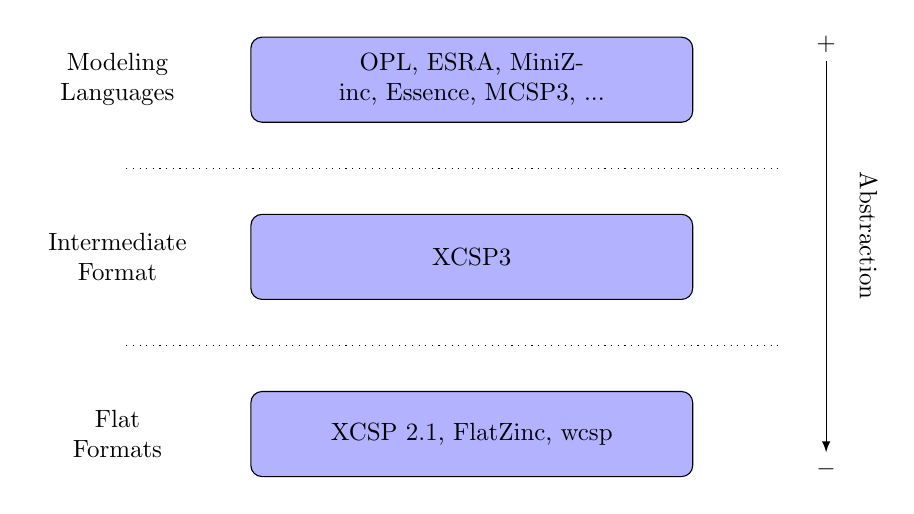
\begin{tikzpicture}[scale=0.9, every node/.style={scale=0.9}]
\tikzstyle{sn}=[draw,rounded corners,minimum height=12mm,fill=blue!30,text width=6cm,text centered]
\node[draw=none,text centered,text width=2.3cm] (1) at (0,0) {Modeling Languages}; 
\node[draw=none,text centered,text width=2.3cm] (2) at (0,-2.5) {Intermediate\\ Format}; 
\node[draw=none,text centered,text width=2.3cm] (2) at (0,-5) {Flat\\ Formats}; 
\node[draw=none] (l) at (0,-1.25) {};
\node[draw=none] (r) at (9.5,-1.25) {};
\node[draw=none] (l2) at (0,-3.75) {};
\node[draw=none] (r2) at (9.5,-3.75) {};
\node[draw=none] (a1) at (10,0.5) {$+$};
\node[draw=none] (a2) at (10,-5.5) {$-$};
\node[sn] (a) at (5,0) {OPL, ESRA, MiniZinc, Essence, MCSP3, ...}; 
\node[sn] (b) at (5,-2.5) {XCSP3}; 
\node[sn] (c) at (5,-5) {XCSP 2.1, FlatZinc, wcsp}; 
\draw[->,>=latex] (a1) -- (a2);
\node[draw=none,rotate=-90] at (10.6,-2.2) {Abstraction};
\draw[dotted] (l) -- (r);
\draw[dotted] (l2) -- (r2);
\end{tikzpicture}
\end{center}
\caption{Modeling Languages, Intermediate and Flat Formats.\label{fig:modfor}}
 \end{figure}



\noindent The complete chain of production, called MCSP3-XCSP3, has many advantages:
\begin{itemize}
\item JSON, Java and XML are robust mainstream technologies
\item Using JSON for data permits to have a unified notation, easy to read for both humans and machines
\item using Java 8 for modeling permits the user to avoid learning again a new programming language
\item Using a coarse-grained XML structure permits to have quite readable problem descriptions, easy to read for both humans and machines
\end{itemize}

{\bf Remark.} Using JSON instead of XML for representing instances is possible but has some drawbacks, as explained in an appendix of XCSP3 Specifications. 

\bigskip
Currently, this is second official release of MCSP3 (with its compiler).
It is available on github: \href{https://github.com/xcsp3team/XCSP3-Java-Tools}{https://github.com/xcsp3team/XCSP3-Java-Tools}, in package \texttt{modeler}.
    

\section{Single Problems}

We propose to start discovering the API with some simple case studies.

\subsection{A Simple Riddle}

Remember that when you were young, you were used to play at riddles, some of them having a mathematical background as for example:
\begin{quote}
{\em Which sequence of successive four integer numbers sum up to 14?}
\end{quote}

\begin{center}
  \includegraphics[scale=0.3]{figures/carambar.jpg}
\end{center}

If you were already familiar with Mathematics, maybe you were able to formalize this ridlle by:
\begin{itemize}
\item introducing four integer variables:
\begin{itemize}
  \item $x_1 \in \N$, $x_2 \in \N$, $x_3 \in \N$, $x_4 \in \N$
\end{itemize}
\item introducing the following mathematical relations (constraints):
\begin{itemize}
\item $x_1+1 = x_2$
\item $x_2+1 = x_3$
\item  $x_3+1=x_4$
\item $x_1 + x_2 + x_3 + x_4 = 14$
\end{itemize}
\end{itemize}

This is a CSP (Constraint Satisfaction problem) instance, involving four integer variables, three binary constraints (i.e., constraints involving exactly two distinct variables) and one quaternary constraint (i.e., constraint involving exactly four distinct variables).

After a rough analysis, we can decide to set 0 as lower bound and 14 as upper bound for the possible values of the integer variables (because, this way, we are absolutely certain of not losing any solutions).
We then obtain the following model in \mt:

\begin{lstlisting}
ç\befç
class Riddle implements ProblemAPI {

  public void model() {
    Var x1 = var("x1", dom(range(15)));
    Var x2 = var("x2", dom(range(15)));
    Var x3 = var("x3", dom(range(15)));
    Var x4 = var("x4", dom(range(15)));
    
    equal(add(x1, 1), x2);
    equal(add(x2, 1), x3);
    equal(add(x3, 1), x4);
    equal(add(x1, x2, x3, x4), 14);
  }
}
ç\aftç
\end{lstlisting}

As you can observe, you just need to build a Java class that implements the interface \nn{ProblemAPI} and that contains a method \nn{model()}.
Within this method, to declare a stand-alone variable, you have to call one of the following methods \nn{var()}: 

\begin{quote}
\begin{myvb}
Var var(String id, Dom dom) 
Var var(String id, Dom dom, String note)

VarSymbolic var(String id, DomSymbolic dom) 
VarSymbolic var(String id, DomSymbolic dom, String note)
\end{myvb}
\end{quote}

As you can imagine, \nn{Var} and \nn{VarSymbolic} are the classes in the API used to represent respectively integer and symbolic variables\footnote{Support for real, set and graph variables will be proposed in a future version of the API.}.
The specified id is the identification of the variable; it is mandatory and must be unique.
Most of the time, the name we give for the Java local variable is the same as the value of its id: for example, note that $x_1$ is the name of a Java variable (whose class is \nn{Var}) that has "$x_1$" as id.
But this is not required.
The ``optional'' parameter \nn{note} is a short comment that can be useful to describe the role of the variable.
For example, if we want ``x1 is the first variable of the sequence'' as comment in the \xt file that can be generated from this \mt model (very soon, we shall see this in action), we have to replace the first statement in Method \nn{model()} above with:

\begin{quote}
\begin{myvb}
Var x1 = var("x1", dom(range(15)), "x1 is the first variable of the sequence");
\end{myvb}
\end{quote}

Now, the question is: how can we build integer and symbolic domains? % (objects from classes \nn{XDomInteger} and \nn{XDomSymbolic})?
For building integer domains, you can call the following methods \nn{dom()}, since each one returns an object from class \nn{Dom}: 
\begin{quote}
\begin{myvb}
Dom dom(int[] values)
Dom dom(int value1, int... otherValues) 
Dom dom(Collection<Integer> values)
Dom dom(IntStream values) 
Dom dom(int[][] m) 
Dom dom(Range range) 
\end{myvb}
\end{quote}

For building symbolic domains, you can call the following methods \nn{dom()}, since each one returns an object from class \nn{DomSymbolic}: 
\begin{quote}
\begin{myvb}
DomSymbolic dom(String[] values)
DomSymbolic dom(String value1, String... otherValues) 
\end{myvb}
\end{quote}

It is important to note that the sixth method above for building an integer domain requires an object Range that can be obtained with one of the following methods \nn{range()}: 
\begin{quote}
\begin{myvb}
Range range(int startInclusive, int endExclusive, int step) 
Range range(int startInclusive, int endExclusive) 
Range range(int length) 
\end{myvb}
\end{quote}
or one of the following methods \nn{rangeClosed()}: 
\begin{quote}
\begin{myvb}
Range rangeClosed(int startInclusive, int endInclusive, int step) 
Range rangeClosed(int startInclusive, int endInclusive) 
\end{myvb}
\end{quote}

Note that the methods \nn{range()} are defined similarly to those introduced for languages Python and JavaScript (from package Lodash), and also for Java IntStream.

\begin{remark}
  Important: the methods \nn{range()} from version 1.0 are now called \nn{rangeClosed()}.
\end{remark}
  
As an illustration, the following table shows which domains are obtained for various calls.
It is important to note that integer domains are systematically sorted and 'made distinct' (i.e., without any two occurences of the same value).

\medskip\begin{tabular}{ll}
\toprule
Call & Domain \\
\midrule
\verb!dom(0,1)! & $\{0,1\}$  \\
\verb!dom(1,2,5,10)! & $\{1,2,5,10\}$  \\
\verb!dom(1,2,5,10,2,4)! & $\{1,2,4,5,10\}$  \\
\verb!dom(new int[] {2,3,4})! & $\{2,3,4\}$  \\
\verb!dom(new int[][] {{1,3},{2,2},{4,6}})! & $\{1,2,3,4,6\}$  \\
\verb!dom(range(5))! & $\{0,1,2,3,4\}$  \\
\verb!dom(range(10,15))! & $\{10,11,12,13,14\}$  \\
\verb!dom(rangeClosed(10,15))! & $\{10,11,12,13,14,15\}$  \\
\verb!dom(range(1,10,3))! & $\{1,4,7\}$  \\
\verb!dom(rangeClosed(1,10,3))! & $\{1,4,7,10\}$  \\
\verb!dom("red","green","blue")! & $\{$``red'',''green'',''blue''$\}$  \\
\bottomrule
\end{tabular}
\bigskip

Now, let us consider the constraints.
Here, we only use intensional constraints.
To build a constraint \gb{intension}, you have to call the method \nn{intension()} with an object \nn{XNodeParent} as parameter for representing the tree-shaped Boolean expression.

\begin{quote}
\begin{myvb}
intension(XNodeParent<IVar> tree) 
\end{myvb}
\end{quote}

Don't be afraid by the type of the parameter. You will never have to handle it explicitly because to build  a tree, all classical operators can be used.
More precisely, all the following methods returns an object \nn{XNodeParent<IVar>}:
\begin{quote}
\begin{myvb}
neg(Object operand) 
abs(Object operand) 
add(Object... operands) 
sub(Object operand1, Object operand2) 
mul(Object... operands) 
div(Object operand1, Object operand2) 
mod(Object operand1, Object operand2) 
sqr(Object operand) {
pow(Object operand1, Object operand2) 
min(Object... operands) 
max(Object... operands) 
dist(Object operand1, Object operand2) 

lt(Object operand1, Object operand2) 
le(Object operand1, Object operand2) 
ge(Object operand1, Object operand2) 
gt(Object operand1, Object operand2) 
ne(Object... operands) 
eq(Object... operands) 

set(Object... operands) 
set(int[] operands) 
in(Object var, Object set) 

not(Object operand) 
and(Object... operands) 
or(Object... operands) 
xor(Object... operands) 
iff(Object... operands) 
imp(Object operand1, Object operand2) 

ifThenElse(Object operand1, Object operand2, Object operand3) 
\end{myvb}
\end{quote}

The precise semantics of these operators is given by Table \ref{tab:semanticsi} in Appendix \ref{app:ops}.


At this point, one may wonder if the constraints of our model should have been declared as:

\begin{quote}
\begin{myvb}
intension(eq(add(x1, 1), x2));
intension(eq(add(x2, 1), x3));
intension(eq(add(x3, 1), x4));
intension(eq(add(x1, x2, x3, x4), 14));
\end{myvb}
\end{quote}

This is correct, indeed.
However, there are some methods in the API that allow us to simplify the expression of some intensional constraints.
This is shown by the following table.

\medskip\begin{tabular}{ll}
  \toprule
Normal Form & Simplified Form \\
  \midrule
  \verb!intension(lt(...))! & \verb!lessThan(...)!  \\
  \verb!intension(le(...))! & \verb!lessEqual(...)!  \\
  \verb!intension(ge(...))! & \verb!greaterEqual(...)!  \\
  \verb!intension(gt(...))! & \verb!greaterThan(...)!  \\
  \verb!intension(eq(...))! & \verb!equal(...)!  \\
  \verb!intension(ne(...))! & \verb!different(...)!  \\
  \verb!intension(in(...))! & \verb!belong(...)!  \\
  \verb!intension(imp(...))! & \verb!implication(...)!  \\
  \verb!intension(iff(...))! & \verb!equivalence(...)!  \\
  \verb!intension(and(...))! & \verb!conjunction(...)!  \\
  \verb!intension(or(...))! & \verb!disjunction(...)!  \\
\bottomrule
\end{tabular}
\bigskip


\begin{remark}
  The shortcut method \nn{different()} was called  \nn{notEqual()} in version 1.0.
\end{remark}

Once you have an \mt model, you can compile it in order to get an \xt file that can be given to a constraint solver.
The command is as follows\footnote{You may need to prefix the name of the class with the relevant package information. For example, if Riddle is in package \texttt{problems.puzz}, you have to write \texttt{java org.xcsp.modeler.Compiler problems.puzz.Riddle}}:
\begin{quote}
\begin{myvb}
java org.xcsp.modeler.Compiler Riddle
\end{myvb}
\end{quote}
The content of the \xt file is: 
\begin{lstlisting}
ç\befç
<instance format="XCSP3" type="CSP">
  <variables>
    <var id="x1"> 0..14 </var>
    <var id="x2"> 0..14 </var>
    <var id="x3"> 0..14 </var>
    <var id="x4"> 0..14 </var>
  </variables>
  <constraints>
    <intension> eq(add(x1,1),x2) </intension>
    <intension> eq(add(x2,1),x3) </intension>
    <intension> eq(add(x3,1),x4) </intension>
    <intension> eq(add(x1,x2,x3,x4),14) </intension>
  </constraints>
  </instance>
ç\aftç
\end{lstlisting}

The variables of our problem (instance) have been declared independently, but it is possible to declare them in a one-dimensional array.
This gives:

\begin{lstlisting}
ç\befç
class Riddle2 implements ProblemAPI {

  public void model() {
    Var x[] = array("x", size(4), dom(range(15)), "x[i] is the ith integer of the sequence");
    
    equal(add(x[0], 1), x[1]);
    equal(add(x[1], 1), x[2]);
    equal(add(x[2], 1), x[3]);
    equal(add(x[0], x[1], x[2], x[3]), 14);
  }
}
ç\aftç
\end{lstlisting}
and the \xt file obtained after compilation:
\begin{quote}
\begin{myvb}
java org.xcsp.modeler.Compiler Riddle2
\end{myvb}
\end{quote}
is:
\begin{lstlisting}
ç\befç
<instance format="XCSP3" type="CSP">
  <variables>
    <array id="x" note="x[i] is the ith integer of the sequence" size="[4]"> 0..14 </array>
  </variables>
  <constraints>
    <intension> eq(add(x[0],1),x[1]) </intension>
    <intension> eq(add(x[1],1),x[2]) </intension>
    <intension> eq(add(x[2],1),x[3]) </intension>
    <intension> eq(add(x[0],x[1],x[2],x[3]),14) </intension>
  </constraints>
</instance>
ç\aftç
\end{lstlisting}

Here, we declare a one-dimensional array of variables: its id is ``x'', its size (length) is 4 and each of its variables has $\{0,1,\dots,14\}$ as domain.
Note that indexing starts at 0.
The methods for declaring one-dimensional arrays of integer or symbolic variables are:

\begin{quote}
\begin{myvb}
Var[] array(String id, Size1D size, Dom dom) 
Var[] array(String id, Size1D size, Dom dom, String note) 
Var[] array(String id, Size1D size, IntToDom f) 
Var[] array(String id, Size1D size, IntToDom f, String note) 

VarSymbolic[] arraySymbolic(String id, Size1D size, DomSymbolic dom) 
VarSymbolic[] arraySymbolic(String id, Size1D size, DomSymbolic dom, String note)
VarSymbolic[] arraySymbolic(String id, Size1D size, IntToDomSymbolic f) 
VarSymbolic[] arraySymbolic(String id, Size1D size, IntToDomSymbolic f, String note)
\end{myvb}
\end{quote}

where all methods require an object \nn{Size1D} that can be simply obtained by calling the following method (this is syntactic sugar):
\begin{quote}
\begin{myvb}
size(int length)
\end{myvb}
\end{quote}

Some of these methods accept lambda functions in order to let the user the possibility of declaring (in the same array) variables with different domains.
For example, suppose that we have analytically deduced that the two first variables of the array must be assigned a value strictly less than 6 and the two last variables of the array must be assigned a value strictly less than 9.
We can write:

\begin{lstlisting}
ç\befç
class Riddle3 implements ProblemAPI {

  public void model() {
    Var x[] = array("x", size(4), i -> i < 2 ? dom(range(6)) : dom(range(9)));
    
    equal(add(x[0], 1), x[1]);
    equal(add(x[1], 1), x[2]);
    equal(add(x[2], 1), x[3]);
    equal(add(x[0], x[1], x[2], x[3]), 14);
  }
}
ç\aftç
\end{lstlisting}
and the \xt file obtained after compilation is:
\begin{lstlisting}
ç\befç
<instance format="XCSP3" type="CSP">
  <variables>
    <array id="x" size="[4]">
      <domain for="x[0] x[1]"> 0..5 </domain>
      <domain for="x[2] x[3]"> 0..8 </domain>
    </array>
  </variables>
  <constraints>
    <intension> eq(add(x[0],1),x[1]) </intension>
    <intension> eq(add(x[1],1),x[2]) </intension>
    <intension> eq(add(x[2],1),x[3]) </intension>
    <intension> eq(add(x[0],x[1],x[2],x[3]),14) </intension>
  </constraints>
</instance>
ç\aftç
\end{lstlisting}

Let us keep analysing the code of the model.
Because the three binary constraints are similar, one may wonder if we couldn't post these constraints in a group (loop).
This is indeed possible by using the following method:

\begin{quote}
\begin{myvb}
forall(Range range, IntConsumer c) 
\end{myvb}
\end{quote}


The behaviour is as follows: the specified consumer object is called for each value in the specified range, and most of the time the goal is to post a constraint when it is called.
Let us see this in action:

\begin{lstlisting}
ç\befç
class Riddle4 implements ProblemAPI {

  public void model() {
    Var x[] = array("x", size(4), dom(range(15)));
    
    forall(range(3), i -> equal(add(x[i], 1), x[i + 1]));

    equal(add(x[0], x[1], x[2], x[3]), 14);
  }
}
ç\aftç
\end{lstlisting}
and the \xt file obtained after compilation is:
\begin{lstlisting}
ç\befç
<instance format="XCSP3" type="CSP">
  <variables>
    <array id="x" size="[4]"> 0..14 </array>
  </variables>
  <constraints>
    <group>
      <intension> eq(add(%0,%1),%2) </intension>
      <args> x[0] 1 x[1] </args>
      <args> x[1] 1 x[2] </args>
      <args> x[2] 1 x[3] </args>
    </group>
    <intension> eq(add(x[0],x[1],x[2],x[3]),14) </intension>
  </constraints>
</instance>
ç\aftç
\end{lstlisting}

Because of the call to the method \nn{forall()}, we obtain a group of constraints in \xt: basically, we have a constraint template with several parameters identified by \%,
and one ``concrete'' constraint per element \xml{args} providing the effective arguments.
For more information about groups in \xt, see Chapter 10 in \href{http://www.xcsp.org/format3.pdf}{\xt Specifications}.
Of course, you can use the classical control structures of Java. So, an alternative way of writting the model is:
\begin{lstlisting}
ç\befç
class Riddle4b implements ProblemAPI {

  public void model() {
    Var x[] = array("x", size(4), dom(range(15)));
    
    for (int i = 0; i < 3; i++)
      equal(add(x[i], 1), x[i + 1]);
    equal(add(x[0], x[1], x[2], x[3]), 14);
  }
}
ç\aftç
\end{lstlisting}
and the \xt file obtained after compilation is:
\begin{lstlisting}
ç\befç
<instance format="XCSP3" type="CSP">
  <variables>
    <array id="x" size="[4]"> 0..14 </array>
  </variables>
  <constraints>
    <intension> eq(add(x[0],1),x[1]) </intension>
    <intension> eq(add(x[1],1),x[2]) </intension>
    <intension> eq(add(x[2],1),x[3]) </intension>
    <intension> eq(add(x[0],x[1],x[2],x[3]),14) </intension>
  </constraints>
</instance>
ç\aftç
\end{lstlisting}

As you can see, the structure is less ovbvious: the group composed of three constraints is no more visible.
We believe that it is a drawback, and consequently, we do prefer to use the method \nn{forall()}.
Nevertheless, notice that it is possible to tune some parameters of the compiler for {\em partially} building groups in an automatic way.  

Finally, it seems more appropriate to represent the last constraint as a constraint \gb{sum}. There are many ways to post a constraint \gb{sum}, as you can see in the Javadoc of the class \texttt{ProblemAPI}.
This gives:

\begin{lstlisting}
ç\befç
class Riddle5 implements ProblemAPI {

  public void model() {
    Var x[] = array("x", size(4), dom(range(15)));
    
    forall(range(3), i -> equal(add(x[i], 1), x[i + 1]));
    sum(x, EQ, 14);
  }
}
ç\aftç
\end{lstlisting}
and the \xt file obtained after compilation is:
\begin{lstlisting}
ç\befç
<instance format="XCSP3" type="CSP">
  <variables>
    <array id="x" size="[4]"> 0..14 </array>
  </variables>
  <constraints>
    <group>
      <intension> eq(add(%0,%1),%2) </intension>
      <args> x[0] 1 x[1] </args>
      <args> x[1] 1 x[2] </args>
      <args> x[2] 1 x[3] </args>
    </group>
    <sum>
      <list> x[] </list>
      <condition> (eq,14) </condition>
    </sum>
  </constraints>
</instance>
ç\aftç
\end{lstlisting}



\subsection{Playing with Small Constraint Networks}

When studying properties of constraint networks, it is frequent to draw some small constraint networks under the form of compatibility graphs (also called microstructure).
For example, Figure \ref{fig:small} presents the compatibility graph of a small constraint network $P$ such that:
\begin{itemize}
\item the set of variables of $P$ is $\f{vars}(P)=\{x,y,z\}$, each variable having $\{a,b\}$ as domain;
  \item the set of constraints of $P$ is $\f{ctrs}(P)= \{\langle x,y \rangle \in \{(a,a),(b,b)\}, \langle x,z \rangle \in \{(a,a),(b,b)\},\langle y,z \rangle \in \{(a,b),(b,a)\}$.
\end{itemize}

\begin{figure}[h!]
\begin{center}
  \includegraphics[scale=1]{figures/ACvsPIC.pdf}
\end{center}
\caption{The compatibility graph of a small constraint network.\label{fig:small}}
\end{figure}

The interested reader can observe that the constraint network is arc-consistent (AC) but not path-inverse consistent (PIC).
Don't worry! It doesn't matter here if you do not know anything about these properties. 
Anyway, the \mt model for our problem is as follows:


\begin{lstlisting}
ç\befç
class Pic implements ProblemAPI {
  
  public void model() {
    VarSymbolic x = var("x", dom("a", "b"));
    VarSymbolic y = var("y", dom("a", "b"));
    VarSymbolic z = var("z", dom("a", "b"));
    
    extension(vars(x, y), tableSymbolic("(a,a)(b,b)"));
    extension(vars(x, z), tableSymbolic("(a,a)(b,b)"));
    extension(vars(y, z), tableSymbolic("(a,b)(b,a)"));
  }
}
ç\aftç
\end{lstlisting}
For compiling it, we execute:
\begin{quote}
\begin{myvb}
java org.xcsp.modeler.Compiler Pic
\end{myvb}
\end{quote}
and the \xt file obtained after compilation is:
\begin{lstlisting}
ç\befç
<instance format="XCSP3" type="CSP">
  <variables>
    <var id="x" type="symbolic"> a b </var>
    <var id="y" type="symbolic"> a b </var>
    <var id="z" type="symbolic"> a b </var>
  </variables>
  <constraints>
    <extension>
      <list> x y </list>
      <supports> (a,a)(b,b) </supports>
    </extension>
    <extension>
      <list> x z </list>
      <supports> (a,a)(b,b) </supports>
    </extension>
    <extension>
      <list> y z </list>
      <supports> (a,b)(b,a) </supports>
    </extension>
  </constraints>
</instance>
ç\aftç
\end{lstlisting}

Here, we declare three stand-alone symbolic variables (note how the domain of each of them is simply composed of the two symbols "a" and "b").
And we declare three binary constraints \gb{extension}. First, note that the scope of the constraints is specified using the method \nn{vars()}.
The many overloading versions of \nn{vars()} permit to build 1-dimensional arrays of variables from a sequence of parameters, where each element of the sequence can be variables, arrays (of any dimension), collections and streams.
All variables are collected in order, and concatenated to form a 1-dimensional array (note that null values are simply discarded).

For posting non-unary extensional constraints (i.e., extensional constraints involving at least two variables), you can use:

\begin{quote}
\begin{myvb}
extension(Var[] scp, int[]... tuples)
extension(Var[] scp, int[][] tuples, Boolean positive) 
extension(Var[] scp, Collection<int[]> tuples)
extension(Var[] scp, Collection<int[]> tuples, Boolean positive) 
extension(Var[] scp, Table table) 

extension(VarSymbolic[] scp, String[]... tuples)
extension(VarSymbolic[] scp, String[][] tuples, Boolean positive) 
extension(VarSymbolic[] scp, TableSymbolic table) 
\end{myvb}
\end{quote}

For unary extensional constraints, you can use:

\begin{quote}
\begin{myvb}
extension(Var x, int... values)
extension(Var x, int[] values, Boolean positive) 

extension(VarSymbolic x, String... values)
extension(VarSymbolic x, String[] values, Boolean positive) 
\end{myvb}
\end{quote}
When the parameter \nn{positive} is present, it indicates if the constraint enumerates the allowed tuples (value $true$) of the forbidden tuples (value $false$).
By default, table constraints are positive.
%Note that it is possible to post unary constraints and non-unary constraints.
As you can observe, specifying tuples is made possible under the form of arrays, collections, streams or \nn{TableAbstract} objects\footnote{\nn{TableAbstract} is the superclass of \nn{Table} and \nn{TableSymbolic}.}.
For building \nn{Table} objects, you can use: 

\begin{quote}
\begin{myvb}
table()                               // empty table
table(int value, int... otherValues)  // only one tuple
table(int[]... tuples)                // several tuples
table(Collection<int[]> tuples        // a collection of tuples
table(Stream<int[]> tuples)           // a stream of tuples
table(Table table)                    // copy of a table
table(String tuples)                  // tuples given in literal String form
\end{myvb}
\end{quote}

For building \nn{TableSymbolic} objects, you can use: 

\begin{quote}
\begin{myvb}
tableSymbolic()                   // empty table
tableSymbolic(String... tuple)    // only one tuple
tableSymbolic(String[]... tuples) // several tuples 
tableSymbolic(String tuples)      // tuples given in literal String form
\end{myvb}
\end{quote}

When modeling, it is usually convenient to use the last method above where tuples are given exactly as they are represented in \xt.
Indeed, with this method, instead of writting:
\begin{quote}
  \verb!extension(vars(x, y), new String[][] {{"a", "a"},{"b", "b"}});!
\end{quote}
we can simply write:
\begin{quote}
  \verb!extension(vars(x, y), tableSymbolic("(a,a)(b,b)"));!
\end{quote}

We could have also written:
\begin{quote}
  \verb!extension(vars(x, y), tableSymbolic().add("a", "a").add("b", "b"));!
\end{quote}
by using the method \nn{add()} of the built symbolic table.

  
Note that there are several methods in classes \nn{TableAbstract}, \nn{Table} and \nn{TableSymbolic} to build ``complex'' tables in several steps: these methods allow method chaining, most of the time, as illustrated by the method \nn{add()} above.
%You also indicate if the table is positive or negative.

Now, suppose that instead of declaring symbolic variables, you prefer to declare integer variables.
By replacing "a" by 0 and "b" by 1, you can write:

\begin{lstlisting}
ç\befç
class Pic2 implements ProblemAPI {
  
  public void model() {
    Var x = var("x", dom(0, 1));
    Var y = var("y", dom(0, 1));
    Var z = var("z", dom(0, 1));
    
    extension(vars(x, y), table("(0,0)(1,1)"));
    extension(vars(x, z), table("(0,0)(1,1)"));
    extension(vars(y, z), table("(0,1)(1,0)"));
  }
}
ç\aftç
\end{lstlisting}
which, when compiled, gives:
\begin{lstlisting}
ç\befç
<instance format="XCSP3" type="CSP">
  <variables>
    <var id="x"> 0 1 </var>
    <var id="y"> 0 1 </var>
    <var id="z"> 0 1 </var>
  </variables>
  <constraints>
    <extension>
      <list> x y </list>
      <supports> (0,0)(1,1) </supports>
    </extension>
    <extension>
      <list> x z </list>
      <supports> (0,0)(1,1) </supports>
    </extension>
    <extension>
      <list> y z </list>
      <supports> (0,1)(1,0) </supports>
    </extension>
  </constraints>
</instance>
ç\aftç
\end{lstlisting}


Again, note that we simply write:
\begin{quote}
  \verb!extension(vars(x, y), table("(0,0)(1,1)"));!
\end{quote}
instead of writting:
\begin{quote}
  \verb!extension(vars(x, y), new int[][] {{0, 0},{1, 1}});!
\end{quote}

We could have also written:
\begin{quote}
  \verb!extension(vars(x, y), table().add(0, 0).add(1, 1));!
\end{quote}
by using the method \nn{add()} of the built integer table.


\section{Academic Problems}

Contrary to single problems, academic problems require the introduction of some pieces of data by the user.


\subsection{Queens}

The problem is stated as follows: can we put 8 queens on a chessboard such that no two queens attack each other?
Two queens attack each other iff they belong to the same row, the same column or the same diagonal.
An illustration is given by Figure \ref{fig:queens}.

\begin{figure}[h]
  \centering
    \begin{subfigure}[t]{0.5\textwidth}
        \centering
        \includegraphics[scale=1]{figures/queen1.pdf}
        \caption{Puzzle}
    \end{subfigure}%
    ~ 
    \begin{subfigure}[t]{0.5\textwidth}
        \centering
        \includegraphics[scale=1]{figures/queen2.pdf}
        \caption{Solution}
    \end{subfigure}
    \caption{Putting 8 queens on a chessboard \label{fig:queens}}
\end{figure}

By considering boards of various size, the problem can be generalized as follows: can we put $n$ queens on a board of size $n \times n$ such that no two queens attack each other?
Contrary to previously introduced single problems, we have to deal here with a family of problem instances, each of them characterized by a distinct value of $n$.
We can try to solve the 8-queens instance, the 10-queens instance, and even the 1000-queens instance.

For such problems, we have to separate the description of the model from the description of the data.
In other words, we have to write a model with some kind of parameters.
In \mt, this is quite natural and easy to do:
\begin{enumerate}
\item clearly identify the parameters of the problem (with their types)
\item introduce fields representing them in the class implementing \nn{ProblemAPI}
\item specify values for these parameters (fields) when you compile to \xt   
\end{enumerate}

In our case, we have only one integer parameter called $n$.
If we associate a variable $q_i$ with the ith row of the board, then we can simply post the following constraints:
\begin{quote}
  $q_i \neq q_j \land |q_i - q_j| \neq |i - j|, \forall i, j : 1 \leq i < j \leq n$
\end{quote}
This is translated as:

\begin{lstlisting}
ç\befç
class Queens implements ProblemAPI {
  int n; // number of queens

  public void model() {
    Var[] q = array("q", size(n), dom(range(n)),
      "q[i] is the column where is put the ith queen (at row i)");
    
    forall(range(n).range(n), (i, j) -> {
      if (i < j)
        conjunction(ne(q[i], q[j]), ne(dist(q[i], q[j]), dist(i, j)));
    });
  }
}
ç\aftç
\end{lstlisting}

Note how we just need to declare the parameter as an integer field $n$ in the class, and how the parameter/field $n$ is used in Method \nn{model()}.
To post the constraints \gb{intension} (remember that \gb{conjunction} is a shortcut method for intensional constraints admitting the operator $and$ at the root of their tree-shaped expressions), we use the following method:

\begin{quote}
\begin{myvb}
forall(Rangesx2 rangesx2, Intx2Consumer c2) 
\end{myvb}
\end{quote}

An object \nn{Rangesx2} represents the Cartesian product of two basic ranges. In our case, it is obtained by:
\begin{quote}
\begin{myvb}
range(n).range(n)
\end{myvb}
\end{quote}
So, when we write:
\begin{quote}
\begin{myvb}
forall(range(n).range(n), (i, j) -> ...
\end{myvb}
\end{quote}
it means: $\forall (i,j) \in 0..n-1 \times 0..n-1$, $\dots$

\bigskip
Now, the question is: how can we solve a specific instance?
The answer is: just compile the model while indicating with the argument \verb!-data=! either the value for $n$ or the name of a JSON file containing an object with a unique field $n$.
In the former case, this gives for $n=4$: 
\begin{quote}
\begin{myvb}
java org.xcsp.modeler.Compiler Queens -data=4
\end{myvb}
\end{quote}
and the \xt file obtained after compilation is:
\begin{lstlisting}
ç\befç
<instance format="XCSP3" type="CSP">
  <variables>
    <array id="q" note="q[i] is the column where is put the ith queen (at row i)" size="[4]">
      0..3
    </array>
  </variables>
  <constraints>
    <group>
      <intension> and(ne(%0,%1),ne(dist(%0,%1),dist(%2,%3))) </intension>
      <args> q[0] q[1] 0 1 </args>
      <args> q[0] q[2] 0 2 </args>
      <args> q[0] q[3] 0 3 </args>
      <args> q[1] q[2] 1 2 </args>
      <args> q[1] q[3] 1 3 </args>
      <args> q[2] q[3] 2 3 </args>
    </group>
  </constraints>
</instance>
ç\aftç
\end{lstlisting}

In the latter case, just build a file ``queens-4.json'' whose content is:
\begin{quote}
\begin{myvb}
{
  "n": 4
}
\end{myvb}
\end{quote}
and execute:
\begin{quote}
\begin{myvb}
java org.xcsp.modeler.Compiler Queens -data=queens-4.json
\end{myvb}
\end{quote}


As already mentioned in the previous section, one could have used classical Java control structures, but remember that it jeopardizes the preservation of the model structure. 

At this point, you have been told that it could be a good idea to post a constraint \gb{allDifferent}.
So, you would like to test a slightly different model, and you think that it is annoying of increasing the number of files (have you observed how many frameworks generate hundreds and even thousands of files; that is crazy!).
Actually, you can put different model variants in the same file by using the method \nn{modelVariant} that accepts a string as parameter.
When you compile, you have then to indicate the name of the variant.
Putting two slightly different model variants in the same file gives:

\begin{lstlisting}
ç\befç
class Queens implements ProblemAPI {
  int n; // number of queens
  
  public void model() {
    Var[] q = array("q", size(n), dom(range(n)));
    
    if (modelVariant("m1")) {
      forall(range(n).range(n), (i, j) -> {
	if (i < j)
	  conjunction(ne(q[i], q[j]), ne(dist(q[i], q[j]), dist(i, j)));
      });
    }
    if (modelVariant("m2")) {
      allDifferent(q);
      forall(range(n).range(n), (i, j) -> {
	if (i < j)
	  different(dist(q[i], q[j]), dist(i, j));
      });
    }
  }
}
ç\aftç
\end{lstlisting}

To compile the first model variant ("m1"), just type:
\begin{quote}
\begin{myvb}
java org.xcsp.modeler.Compiler Queens -variant=m1 -data=4
\end{myvb}
\end{quote}


To compile the second model variant ("m2"), just type:
\begin{quote}
\begin{myvb}
java org.xcsp.modeler.Compiler Queens -variant=m2 -data=4 
\end{myvb}
\end{quote}

For the second model, you obtain:

\begin{lstlisting}
ç\befç
<instance format="XCSP3" type="CSP">
  <variables>
    <array id="q" size="[4]"> 0..3 </array>
  </variables>
  <constraints>
    <allDifferent> q[] </allDifferent>
    <group>
      <intension> ne(dist(%0,%1),dist(%2,%3)) </intension>
      <args> q[0] q[1] 0 1 </args>
      <args> q[0] q[2] 0 2 </args>
      <args> q[0] q[3] 0 3 </args>
      <args> q[1] q[2] 1 2 </args>
      <args> q[1] q[3] 1 3 </args>
      <args> q[2] q[3] 2 3 </args>
    </group>
  </constraints>
</instance>
ç\aftç
\end{lstlisting}

\begin{remark}
  In Version 1.0, \verb!-model=! was used instead of \verb!-variant=!.
\end{remark}

Finally, someone told you that it was possible to post only three constraints \gb{allDifferent} for this problem.
More specifically, for two of them, instead of providing a sequence of variables, you must provide a sequence of trees.
This is related to the concept of view in constraint programming.

After adding the following piece of code:
\begin{lstlisting}
ç\befç
    if (modelVariant("m3")) {
      allDifferent(q);
      allDifferent(treesFrom(range(n), i -> add(q[i], i)));
      allDifferent(treesFrom(range(n), i -> sub(q[i], i)));
    }
ç\aftç
\end{lstlisting}
and compiling this third model variant ("m3") by executing:
\begin{quote}
\begin{myvb}
java org.xcsp.modeler.Compiler Queens -variant=m3 -data=4
\end{myvb}
\end{quote}
we obtain:
\begin{lstlisting}
ç\befç
<instance format="XCSP3" type="CSP">
  <variables>
    <array id="q" size="[4]"> 0..3 </array>
  </variables>
  <constraints>
    <allDifferent> q[] </allDifferent>
    <allDifferent> add(q[0],0) add(q[1],1) add(q[2],2) add(q[3],3) </allDifferent>
    <allDifferent> sub(q[0],0) sub(q[1],1) sub(q[2],2) sub(q[3],3) </allDifferent>
  </constraints>
</instance>
ç\aftç
\end{lstlisting}

Here, we use a method \nn{treesFrom()} that computes a stream of trees (Boolean or integer expressions) by generating a specific tree for each value in the specified range.
Below, this is the fourth method of available similar methods:


\begin{quote}
\begin{myvb}
treesFrom(IntStream stream, Function<Integer, XNodeParent<IVar>> f) 
treesFrom(Collection<Integer> c, Function<Integer, XNodeParent<IVar>> f) 
treesFrom(int[] t, Function<Integer, XNodeParent<IVar>> f) 
treesFrom(Range r, Function<Integer, XNodeParent<IVar>> f) 
\end{myvb}
\end{quote}
%We could have simply chosen to write things with the help of Java 8 streams, just like that:

If ever, when applied on an integer (from a range, array, stream, collection), $null$ is returned by the specified function $f$, this is simply ignored.
%Here, for the sake of conciseness, we use the method \nn{provideObjects()} from Class \nn{Range}.
%Note that other related methods from this class are very useful, and in particular \nn{provideVars()} and \nn{provideVals()}.



\subsection{Board Coloration Problem}

The (chess)board coloration problem is to color all squares of a board composed of $r$ rows and $c$ colomns such that the four corners of any rectangle in the board must not be assigned the same color.
Importantly, we want to minimize the number of used colors.

\begin{figure}[h]
\begin{center}
  \includegraphics[scale=0.1]{figures/chessboardColoration.jpg}
\end{center}
\caption{Coloring Boards.\label{fig:board}}
\end{figure}

This time, we need two integer parameters $r$ and $c$.
After a very rough analysis, we can decide to use $r \times c$ as an upper bound of the number of used colors. 
This gives:


\begin{lstlisting}
ç\befç
class BoardColoration implements ProblemAPI {
  int r; // number of rows 
  int c; // number of columns

  public void model() {
    Var[][] x = array("x", size(r, c), dom(range(r * c)), "x[i][j] is the color at row i and column j");
    
    forall(range(r).range(r).range(c).range(c), (i1, i2, j1, j2) -> {
      if (i1 < i2 && j1 < j2)
        notAllEqual(x[i1][j1], x[i1][j2], x[i2][j1], x[i2][j2]);
    });
    
    minimize(MAXIMUM, x);
  }
}
ç\aftç
\end{lstlisting}

Here, we declare a two-dimensional array of variables: its id is ``x'', its size is $r \times c$ and each of its variables has $\{0,1,\dots,r\times c-1\}$ as domain.
Note that indexing starts at 0.
The methods for declaring two-dimensional arrays of integer variables are:

\begin{quote}
\begin{myvb}
Var[][] array(String id, Size2D size, Dom dom)
Var[][] array(String id, Size2D size, Dom dom, String note)

Var[][] array(String id, Size2D size, Intx2ToDom f)
Var[][] array(String id, Size2D size, Intx2ToDom f, String note) 
\end{myvb}
\end{quote}

where all methods require an object \nn{Size2D} that can be simply obtained by calling the following method:
\begin{quote}
\begin{myvb}
size(int length1, int length2)
\end{myvb}
\end{quote}

To post the constraints \gb{notAllEqual}, we use the following method:

\begin{quote}
\begin{myvb}
forall(Rangesx4 rangesx4, Intx4Consumer c4) 
\end{myvb}
\end{quote}

An object \nn{Rangesx4} represents the Cartesian product of four basic ranges. In our case, it is obtained by:
\begin{quote}
\begin{myvb}
range(r).range(r).range(c).range(c)
\end{myvb}
\end{quote}
So, when we write:
\begin{quote}
\begin{myvb}
forall(range(r).range(r).range(c).range(c), (i1, i2, j1, j2) -> ...
\end{myvb}
\end{quote}
it means: $\forall (i1,i2,j1,j2) \in 0..r-1 \times 0..r-1 \times 0..c-1 \times 0..c-1$, $\dots$

\bigskip
Finally, the objective function corresponds to the minimization of the maximum value taken by any variable in the two-dimensional array $x$.
Because domains are all similar, this is indeed equivalent to minimize the number of used colors.
Here are some of the methods that can be called to post an objective function (when no coefficients are required):

\begin{quote}
\begin{myvb}
minimize(IVar x) 
minimize(TypeObjective type, IVar... list) 
minimize(TypeObjective type, IVar[][] list) 
minimize(TypeObjective type, IVar[][][] list) 

maximize(IVar x) 
maximize(TypeObjective type, IVar... list) 
maximize(TypeObjective type, IVar[][] list) 
maximize(TypeObjective type, IVar[][][] list) 
\end{myvb}
\end{quote}

The specified type must take one of the following value\footnote{See Chapter 3 in \href{http://www.xcsp.org/format3.pdf}{\xt Specifications} for more information.}:
\begin{itemize}
\item EXPRESSION
\item SUM
\item PRODUCT
\item MINIMUM
\item MAXIMUM
\item NVALUES
\item LEX
\end{itemize}


\bigskip
To solve a specific instance, as usually, we have first to compile the model while indicating with the argument \verb!-data=! either the values for $r$ and $c$ or the name of a JSON file containing an object with two fields $r$ and $c$.
In the former case, this gives for $r=3$ and $c=3$: 
\begin{quote}
\begin{myvb}
java org.xcsp.modeler.Compiler BoardColoration -data=[3,3]
\end{myvb}
\end{quote}

As you can observe, you need to use square brackets to surround values sepated by commas (no whitespace authorized).
The \xt file obtained after compilation is:

\begin{lstlisting}
ç\befç
<instance format="XCSP3" type="COP">
  <variables>
    <array id="x" size="[3][3]" note="x[i][j] is the color at row i and column j"> 0..8 </array>
  </variables>
  <constraints>
    <group>
      <nValues>
        <list> %... </list>
        <condition> (gt,1) </condition>
      </nValues>
      <args> x[0][0] x[0][1] x[1][0] x[1][1] </args>
      <args> x[0][0] x[0][2] x[1][0] x[1][2] </args>
      <args> x[0][1] x[0][2] x[1][1] x[1][2] </args>
      <args> x[0][0] x[0][1] x[2][0] x[2][1] </args>
      <args> x[0][0] x[0][2] x[2][0] x[2][2] </args>
      <args> x[0][1] x[0][2] x[2][1] x[2][2] </args>
      <args> x[1][0] x[1][1] x[2][0] x[2]]1] </args>
      <args> x[1][0] x[1][2] x[2][0] x[2][2] </args>
      <args> x[1][1] x[1][2] x[2][1] x[2][2] </args>
    </group>
  </constraints>
  <objectives>
    <minimize type="maximum"> x[][] </minimize>
  </objectives>
</instance>
ç\aftç
\end{lstlisting}

We can also build a file ``board-3-3.json'' whose content is:
\begin{quote}
\begin{myvb}
{
  "r": 3,
  "c": 3
}
\end{myvb}
\end{quote}
and execute:
\begin{quote}
\begin{myvb}
java org.xcsp.modeler.Compiler BoardColoration -data=board-3-3.json
\end{myvb}
\end{quote}


As a matter of fact, this problem has many symmetries.
It is known that we can break variable symmetries by posting a lexicographic constraint between any two successive rows and any two successive columns.
One could post these constraints independently, but it is simpler to post a global constraint \gb{lexMatrix}.
It is relevant to tag this constraint because it clearly informs us that it is used for symmetry breaking: tagging is made possible by calling the method \nn{tag()}, with a string as parameter (here, we use a predefined constant called \texttt{SYMMETRY\_BREAKING}). 
The model is now:

\begin{lstlisting}
ç\befç
class BoardColoration implements ProblemAPI {
  int r; // number of rows 
  int c; // number of columns

  public void model() {
    Var[][] x = array("x", size(r, c), dom(range(r * c)));
    
    forall(range(r).range(r).range(c).range(c), (i1, i2, j1, j2) -> {
      if (i1 < i2 && j1 < j2)
        notAllEqual(x[i1][j1], x[i1][j2], x[i2][j1], x[i2][j2]);
    });
    lexMatrix(x, INCREASING).tag(SYMMETRY_BREAKING);

    minimize(MAXIMUM, x);
  }
}
ç\aftç
\end{lstlisting}

and after compilation, still prodiding two occurrences of 3 as data, we have the following additionnal element in the generated \xt file:

\begin{lstlisting}
ç\befç
    <lex class="symmetryBreaking">
      <matrix> x[][] </matrix>
      <operator> le </operator>
    </lex>
ç\aftç
\end{lstlisting}


Note the presence of the attribute \nn{class} that results from the call to method \nn{tag()}.
Easily, a solver can now solve this instance with or without symmetry breaking.
Indeed, at time of parsing, it is quite easy to discard XML elements with a specified tag (class): this is currently made possible with the available parsers in Java and C++ for \xt.
The interest is that we have only one file, with can be used for testing different model variants. 


\subsection{Magic Sequence}

A magic sequence of order $n$ is a sequence of integers $x_0,\dots,…x_{n-1}$ between 0 and $n-1$, such that each value $i \in 0..n−1$ occurs exactly $x_i$ times in the sequence.
For example,
\begin{quote}
\begin{myvb}
  6 2 1 0 0 0 1 0 0 0
\end{myvb}
\end{quote}
is a magic sequence of order 10 since 0 occurs 6 times, 1 occurs twice, $\dots$ and 9 occurs 0 times.

One can prove that every solution respects:
\begin{quote}
  $x_0 + x_1 + x_2 + x_3 + \dots + x_{n-1} = 0$
\end{quote}
and
\begin{quote}
  $-1x_0 + 0x_1 + 1x_2 + 2x_3 + \dots + (n-2)x_{n-1} = 0$
\end{quote}

So, it may be a good idea to post these additional constraints  and making it clear that they are redundant (i.e., not modifying the set of solutions) by using an appropriate tag.
This gives:

\begin{lstlisting}
ç\befç
class MagicSequence implements ProblemAPI {
  int n; // order of the sequence

  public void model() {
    Var[] x = array("x", size(n), dom(range(n)), "x[i] is the ith value of the sequence");
    
    cardinality(x, range(n), occurExactly(x))
      .note("each value i occurs exactly x[i] times in the sequence");

    block(() -> {
      sum(x, EQ, n);
      sum(x, range(-1, n - 2), EQ, 0);
    }).tag(REDUNDANT_CONSTRAINTS);
  }
}
ç\aftç
\end{lstlisting}

On the one hand, the constraint \gb{cardinality} is exactly what we need here.
We invite the reader to look at the overloaded methods for \gb{cardinality} in Class \nn{ProblemAPI} and see how we can manage occurrences through many methods.
Here, the method we use simply states that each value $i$ in $0..n-1$, given by \verb!range(n)!, must occur exactly $x[i]$ times.
Observe also how we can associate a comment with a constraint by calling methods \nn{note()}.
On the other hand, we have put together the two additional constraints in a so-called block, permitting to tag these two constraints (actually, the block) with the information ``redundantConstraints''.
The method that we have used is:

\begin{quote}
\begin{myvb}
block(Runnable r) 
\end{myvb}
\end{quote}

By the way, note that we can tag any constraint or group of constraints by calling \nn{tag()}.
Now, if we execute:
\begin{quote}
\begin{myvb}
java org.xcsp.modeler.Compiler MagicSequence -data=6
\end{myvb}
\end{quote}
we obtain the following \xt instance:
\begin{lstlisting}
ç\befç
<instance format="XCSP3" type="CSP">
  <variables>
    <array id="x" size="[6]" note="x[i] is the ith value of the sequence"> 0..5 </array>
  </variables>
  <constraints>
    <cardinality note="each value i occurs exactly x[i] times in the sequence">
      <list> x[] </list>
      <values> 0 1 2 3 4 5 </values>
      <occurs> x[] </occurs>
    </cardinality>
    <block class="redundantConstraints">
      <sum>
        <list> x[] </list>
        <condition> (eq,6) </condition>
      </sum>
      <sum>
        <list> x[] </list>
        <coeffs> -1 0 1 2 3 4 </coeffs>
        <condition> (eq,0) </condition>
      </sum>
    </block>
  </constraints>
</instance>
ç\aftç
\end{lstlisting}

\subsection{Golomb Ruler}

This problem (and its variants) is said to have many practical applications including sensor placements for x-ray crystallography and radio astronomy. 
A Golomb ruler may be defined as a set of $n$ integers $0 = a_1 < a_2 < ... < a_n$ such that the $n(n-1)/2$ differences $a_j - a_i$, $1 \leq i < j \leq n$ are distinct. 
Such a ruler is said to contain $n$ marks and is of length $a_n$. 
The objective is to find optimal (minimum length) or near optimal rulers. 
An optimal ruler for $n=4$ is illustrated below:

\begin{center}
\includegraphics[scale=0.4]{figures/GolombRuler4.png} 
\end{center}

Dimitromanolakis has computed relatively short Golomb rulers
and thus showed with computer aid that the optimal ruler for $n \leq 65,000$ has length less than $n^2$.

One possible model (variant) involves auxiliary variables, and ternary constraints.
We choose this model because it allows us to introduce decision variables (the way to define them in MCSP3).
The model is:

\begin{lstlisting}
ç\befç
class GolombRuler implements ProblemAPI {
  int n; // order of the problem

  public void model() {
    int rulerLength = n * n; // an upperbound

    Var[] x = array("x", size(n), dom(range(rulerLength+1)),
      "x[i] is the position of the ith tick");
    Var[][] y = array("y", size(n, n), (i, j) -> dom(range(1, rulerLength)).when(i < j),
      "y[i][j] is the distance between x[i] and x[j]");
      
    allDifferent(y);
    forall(range(n).range(n), (i, j) -> {
      if (i < j)
        equal(x[j], add(x[i], y[i][j]));
    }).note("Linking variables of arrays x and y");
      
    block(() -> {
      equal(x[0], 0);
      strictlyIncreasing(x);
    }).tag(SYMMETRY_BREAKING);
    
    minimize(x[x.length-1]);

    decisionVariables(x);
  }
}
ç\aftç
\end{lstlisting}

First, observe that we declare a two-dimensional array of variables, called $y$, even if only a part of this array will really contain variables.
This is handled by the lambda function that returns a domain only when $ i \geq j$ by calling the method \nn{when()}.
This way, we can simply post a constraint \gb{allDifferent} by specifying the array $y$ (even if it contains \texttt{null} in some cells).

Concerning the decision variables (those that when assigned identify a complete instantiation), we just have to call the method \nn{decisionVariables()}.
In our case, the array $x$ denotes the decision variables.

By executing:
\begin{quote}
\begin{myvb}
java org.xcsp.modeler.Compiler GolombRuler -data=3
\end{myvb}
\end{quote}
we obtain:
\begin{lstlisting}
ç\befç
<instance format="XCSP3" type="COP">
  <variables>
    <array id="x" note="x[i] is the position of the ith tick" size="[3]"> 0..9 </array>
    <array id="y" note="y[i][j] is the distance between x[i] and x[j]" size="[3][3]"> 1..9 </array>
  </variables>
  <constraints>
    <allDifferent> y[0][1..2] y[1][2] </allDifferent>
    <group note="Linking variables of arrays x and y">
      <intension> eq(%0,add(%1,%2)) </intension>
      <args> x[1] x[0] y[0][1] </args>
      <args> x[2] x[0] y[0][2] </args>
      <args> x[2] x[1] y[1][2] </args>
    </group>
    <block class="symmetryBreaking">
      <ordered>
        <list> x[] </list>
        <operator> lt </operator>
      </ordered>
      <intension> eq(x[0],0) </intension>
    </block>
  </constraints>
  <objectives>
    <minimize> x[2] </minimize>
  </objectives>
  <annotations>
    <decision> x[] </decision>
  </annotations>
</instance>
ç\aftç
\end{lstlisting}



\section{Structured Problems}

Some problems need more than elementary data, that is more than a few elementary pieces of data such as integers. 
Here, we call them structured problems for simplicity.

\subsection{Sudoku}

\begin{figure}[h]
  \centering
    \begin{subfigure}[t]{0.5\textwidth}
        \centering
        \includegraphics[scale=1]{figures/sudoku1.pdf}
        \caption{Puzzle}
    \end{subfigure}%
    ~ 
    \begin{subfigure}[t]{0.5\textwidth}
        \centering
        \includegraphics[scale=1]{figures/sudoku2.pdf}
        \caption{Solution}
    \end{subfigure}
    \caption{Solving a Sudoku Grid\label{fig:sudoku}}
\end{figure}

This well-known problem is stated as follows: fill in a grid using digits ranging from 1 to 9 such that:
\begin{itemize}
\item all digits occur on each row
\item all digits occur on each column
  \item all digits occur in each $3 \times 3$ block (starting at a position multiple of 1) 
\end{itemize}
An illustration is given by Figure \ref{fig:sudoku}.

Because there are several clues, and because their number cannot be anticipated, we need a parameter \texttt{clues} that represents a two-dimensional array of integer values.
When $\texttt{clues}[i][j]$ is 0, it means that the cell is empty, whereas when it contains a digit between 1 and 9, it means that it represents a fixed value (clue).
The model we can write is then:


\begin{lstlisting}
ç\befç
class Sudoku implements ProblemAPI {
  int[][] clues; // if not 0, clues[i][j] is a value imposed at row i and col j

  public void model() {
    Var[][] x = array("x", size(9, 9), dom(rangeClosed(1, 9)));

    allDifferentMatrix(x);
    forall(range(0, 8, 3).range(0, 8, 3),
      (i, j) -> allDifferent(select(x, range(i, i + 2).range(j, j + 2)))).tag(BLOCKS);
    instantiation(x, clues, onlyOn((i, j) -> clues[i][j] != 0)).tag(CLUES);
  }
}
ç\aftç
\end{lstlisting}

To ensure that all digits are different on each row and each column, we use:

\begin{quote}
\begin{myvb}
allDifferentMatrix(Var[][] matrix) 
\end{myvb}
\end{quote}

Then, we have to post a constraint \gb{allDifferent} on each block.
Note how we use the following method \nn{select()}, which builds a one-dimensional array of variables by selecting those from the specified two-dimensional array of variables that respect the specified double range:

\begin{quote}
\begin{myvb}
select(T[][] vars, Rangesx2 rangesx2) 
\end{myvb}
\end{quote}

This allows us to extract the right subset of 9 variables for each block.

Finally, each clue (given value) represents a unary constraint.
We can post them using the constraint \gb{instantiation}.
The method that we use here is:

\begin{quote}
\begin{myvb}
instantiation(Var[][] list, int[][] values, Intx2Predicate p) 
\end{myvb}
\end{quote}
that permits to assign the variable $list[i][j]$ with the value $values[i][j]$ provided that $p$ returns true for $(i,j)$.
Note how we use syntactic sugar here, by calling the method \nn{onlyOn()} that simply returns its parameter.
We also tag the group of block constraints as well as the constraint posting clues.


Suppose now that we have a file 'grid.json'' containing:
\begin{quote}
\begin{myvb}
{
  "clues": [
    [0,4,0,0,0,0,0,0,0],
    [5,3,9,0,0,1,0,6,0],
    [0,0,1,0,0,2,0,5,0],
    [4,0,7,2,0,9,0,0,6],
    [0,0,6,0,0,0,5,0,0],
    [8,0,0,6,0,3,1,0,7],
    [0,8,0,7,0,0,2,0,0],
    [0,6,0,3,0,0,4,1,8],
    [0,0,0,0,0,0,0,7,0]
  ]
}
\end{myvb}
\end{quote}
then, we can execute:
\begin{quote}
\begin{myvb}
java org.xcsp.modeler.Compiler Sudoku -data=grid.json
\end{myvb}
\end{quote}
and we obtain the following (simplified here) \xt instance:
\begin{lstlisting}
ç\befç
<instance format="XCSP3" type="CSP">
  <variables>
    <array id="x" size="[9][9]"> 1..9 </array>
  </variables>
  <constraints>
    <allDifferent>
      <matrix> x[][] </matrix>
    </allDifferent>
    <group class="blocks">
      <allDifferent> %... </allDifferent>
      <args> x[0..2][0..2] </args>
      <args> x[0..2][3..5] </args>
      <args> x[0..2][6..8] </args>
      <args> x[3..5][0..2] </args>
      <args> x[3..5][3..5] </args>
      <args> x[3..5][6..8] </args>
      <args> x[6..8][0..2] </args>
      <args> x[6..8][3..5] </args>
      <args> x[6..8][6..8] </args>
    </group>
    <instantiation class="clues" note="Just 2 clues here for the simplicity of the illustration">
      <list> x[0][1] x[8][7] </list>
      <values> 4 7 </values>
    </instantiation>
  </constraints>
</instance>
ç\aftç
\end{lstlisting}

Suppose now that we would like to generate an instance without any clue.
Of course, we can build a grid only containing the value 0, but this is a little bit tedious. 
Actually, you just need to use a JSON file like this:

\begin{quote}
\begin{myvb}
{
  "clues": null
}
\end{myvb}
\end{quote}


\subsection{Warehouse Location Problem}

In the Warehouse Location problem (WLP), a company considers opening warehouses at some candidate locations in order to supply its existing stores.
Each possible warehouse has the same maintenance cost, and a capacity designating the maximum number of stores that it can supply.
Each store must be supplied by exactly one open warehouse.
The supply cost to a store depends on the warehouse.
The objective is to determine which warehouses to open, and which of these warehouses should supply the various stores, such that the sum of the maintenance and supply costs is minimized.
See \href{http://csplib.org/Problems/prob034/}{CSPLib--Problem 034}.

\begin{figure}[h]
\begin{center}
  \includegraphics[scale=0.75]{figures/warehouse.jpg}
\end{center}
\caption{Warehouse.\label{fig:warehouse}}
\end{figure}

An example of data is the file ``warehouse.json'' containing:

{\small
  \begin{quote}
\begin{myvb}
{
  "fixedCost": 30,
  "warehouseCapacities": [1,4,2,1,3],
  "storeSupplyCosts": [
    [100,24,11,25,30],[28,27,82,83,74],[74,97,71,96,70],[2,55,73,69,61],
    [46,96,59,83,4],[42,22,29,67,59],[1,5,73,59,56],[10,73,13,43,96],
    [93,35,63,85,46],[47,65,55,71,95]
  ]
}
\end{myvb}
\end{quote}
}

A possible model is:

\begin{lstlisting}
ç\befç
class Warehouse implements ProblemAPI {
  int fixedCost;
  int[] warehouseCapacities;
  int[][] storeSupplyCosts;
  
  public void model() {
    int nWarehouses = warehouseCapacities.length;
    int nStores = storeSupplyCosts.length;
    
    Var[] s = array("s", size(nStores), dom(range(nWarehouses)),
      "s[i] is the warehouse supplier of store i");
    Var[] c = array("c", size(nStores), i -> dom(storeSupplyCosts[i]),
      "c[i] is the cost of supplying store i");
    Var[] o = array("o", size(nWarehouses), dom(0, 1),
      "o[i] is 1 if the warehouse i is open");
    
    forall(range(nWarehouses),
      i -> atMost(s, takingValue(i), warehouseCapacities[i]));
    forall(range(nStores),
      i -> element(o, at(s[i]), takingValue(1)));
    forall(range(nStores),
      i -> element(storeSupplyCosts[i], at(s[i]), takingValue(c[i])));

    int[] coeffs = vals(repeat(1,nStores),repeat(fixedCost,nWarehouses));
    minimize(SUM, vars(c,o), weightedBy(coeffs)); 
  }
}
ç\aftç
\end{lstlisting}

Here, it is intersting to see how we can define a specific domain to each variable of the array $c$ by means of a simple lambda function.
Remember that values are sorted and made distinct. 
The objective function corresponds to minimizing a weighted sum.
Note how \verb!vars(c,o)! builds a 1-dimensional array from two arrays, and how similarly the method \nn{vals()} concatenates integer values from two arrays to form a 1-dimensional array of integers.
On our example, the array \texttt{coeffs} is \verb!1 1 1 1 1 1 1 1 1 1 30 30 30 30 30! because we have 10 stores and 5 warehouses.
Finally, notice the syntactic sugar offered by methods \nn{takingValue()}, \nn{at()} and \nn{weightedBy()} that simply return the specified parameter (although we could avoid calling these identity functions, this renders the code of the model more readable). 

After executing:
\begin{quote}
\begin{myvb}
java org.xcsp.modeler.Compiler Warehouse -data=warehouse.json
\end{myvb}
\end{quote}
we obtain the following \xt instance (constraints are ommitted):

\begin{lstlisting}
ç\befç
<instance format="XCSP3" type="COP">
  <variables>
    <array id="s" note="s[i] is the warehouse supplier of store i" size="[10]"> 0..4 </array>
    <array id="c" note="c[i] is the cost of supplying store i" size="[10]">
      <domain for="c[0]"> 11 24 25 30 100 </domain>
      <domain for="c[1]"> 27 28 74 82 83 </domain>
      <domain for="c[2]"> 70 71 74 96 97 </domain>
      <domain for="c[3]"> 2 55 61 69 73 </domain>
      <domain for="c[4]"> 4 46 59 83 96 </domain>
      <domain for="c[5]"> 22 29 42 59 67 </domain>
      <domain for="c[6]"> 1 5 56 59 73 </domain>
      <domain for="c[7]"> 10 13 43 73 96 </domain>
      <domain for="c[8]"> 35 46 63 85 93 </domain>
      <domain for="c[9]"> 47 55 65 71 95 </domain>
    </array>
    <array id="o" note="o[i] is 1 if the warehouse i is open" size="[5]"> 0 1 </array>
  </variables>
  <constraints>
    ...
  </constraints>
  <objectives>
    <minimize type="sum">
      <list> c[] o[] </list>
      <coeffs> 1 1 1 1 1 1 1 1 1 1 30 30 30 30 30 </coeffs>
    </minimize>
  </objectives>
</instance>
ç\aftç
\end{lstlisting}


In some occasions, in the class implementing \nn{ProblemAPI} you may wish to define additionnal fields that are not directly concerned by the model, i.e., are not considerered as data/parameters for the model. 
It then suffices to use the Java annotation \nn{@NotData}.

For the sake of illustration (although this renders code a little bit less concise and more obscure), we replace both local variables \texttt{nWarehouses} and \texttt{nStores} by fields in \nn{Warehouse}.
This gives:

\begin{lstlisting}
ç\befç
class Warehouse implements ProblemAPI {
  int fixedCost;
  int[] warehouseCapacities;
  int[][] storeSupplyCosts;

  @NotData
  int nWarehouses;
  @NotData
  int nStores;
  
  public void model() {
    nWarehouses = warehouseCapacities.length;
    nStores = storeSupplyCosts.length;
    
    ... 
ç\aftç
\end{lstlisting}


\subsection{Blackhole}

\begin{figure}[h!]
\begin{center}
  \includegraphics[scale=0.4]{figures/solitaire.png}
\end{center}
\caption{Blackhole.\label{fig:solitaire}}
\end{figure}

From WikiPedia. ``Black Hole is a solitaire card game. Invented by David Parlett, this game's objective is to compress the entire deck into one foundation.
The cards are dealt to a board in piles of three.
The leftover card, dealt first or last, is placed as a single foundation called the Black Hole.
This card usually is the Ace of Spades.
Only the top cards of each pile in the tableau are available for play and in order for a card to be placed in the Black Hole, it must be a rank higher or lower than the top card on the Black Hole. This is the only allowable move in the entire game.
The game ends if there are no more top cards that can be moved to the Black Hole. The game is won if all of the cards end up in the Black Hole.''
An illustration is given by Figure \ref{fig:solitaire}.

We may want to play with various sizes of piles and various number of cards per suit.
An example of data is the file ``blackhole.json'' containing:

{\small
  \begin{quote}
\begin{myvb}
{
  "nCardsPerSuit": 4,
  "nCardsPerPile": 3,
  "piles": [[1,4,13],[15,9,6],[14,2,12],[7,8,5],[11,10,3]]}
}
\end{myvb}
\end{quote}
}

A possible model is:

\begin{lstlisting}
ç\befç
class Blackhole implements ProblemAPI {

  int nCardsPerSuit, nCardsPerPile;
  int[][] piles;

  public void model() {
    int nCards = 4 * nCardsPerSuit;
    int nPiles = (nCards-1) / nCardsPerPile;
    
    Var[] x = array("x", size(nCards), dom(range(nCards)),
      "x[i] is the value j of the card at the ith position of the stack.");
    Var[] y = array("y", size(nCards), dom(range(nCards)),
      "y[j] is the position i of the card whose value is j");
    
    channel(x, y);
    equal(y[0], 0).note("the ace of Spades is initially on the stack");
    
    forall(range(nPiles), i ->
      ordered(variablesFrom(piles[i], j -> y[j]), STRICTLY_INCREASING))
    .note("cards must be played in the order of the piles");

    int[][] tuples = range(nCards).range(nCards).select((i, j) ->
      i%nCardsPerSuit==(j+1)%nCardsPerSuit || j%nCardsPerSuit==(i+1)%nCardsPerSuit);
    slide(x, range(nCards-1), i -> extension(vars(x[i], x[i+1]), tuples))
      .note("each new card on the stack must be at a rank higher or lower than the previous one.");            
  }
}
ç\aftç
\end{lstlisting}  

Note how the constraint \gb{channel} is used to make a channelling between the two arrays $x$ and $y$,
how we can collect variables with \nn{variablesFrom()}, and how tuples are built using an object \nn{Rangesx2} and a lambda function, both given as parameter of the method \nn{select()}.
Finally, we use the meta-constraint \gb{slide} to guarantee that each new card is at a rank higher or lower than the previous one.


After executing:
\begin{quote}
\begin{myvb}
java org.xcsp.modeler.Compiler Blackhole -data=blackhole.json
\end{myvb}
\end{quote}
we obtain the following \xt instance (some tuples have been ommitted; see the presence of the ellipsis $\dots$):


\begin{lstlisting}
ç\befç
<instance format="XCSP3" type="CSP">
  <variables>
  <array id="x" note="x[i] is the value j of the card at the ith pos. of the stack." size="[16]">
    0..15
  </array>
  <array id="y" note="y[j] is the position i of the card whose value is j" size="[16]">
    0..15
  </array>
  </variables>
  <constraints>
    <channel>
      <list> x[] </list>
      <list> y[] </list>
    </channel>
    <intension note="The ace of Spades is initially on the stack"> eq(y[0],0) </intension>
    <group note="We must play in the order of the piles">
      <intension> lt(%0,%1) </intension>
      <args> y[1] y[4] </args>
      <args> y[4] y[13] </args>
      <args> y[15] y[9] </args>
      <args> y[9] y[6] </args>
      <args> y[14] y[2] </args>
      <args> y[2] y[12] </args>
      <args> y[7] y[8] </args>
      <args> y[8] y[5] </args>
      <args> y[11] y[10] </args>
      <args> y[10] y[3] </args>
    </group>
    <slide>
      <list collect="2"> x[] </list>
      <extension>
        <list> %0 %1 </list>
        <supports> (0,1)(0,3)(0,5)(0,7)(0,9)(0,11)...(15,14) </supports>
      </extension>
    </slide>
  </constraints>
</instance>
ç\aftç
\end{lstlisting}  

%In many occasions, you have different ways of posting constraints.
%You should always try to choose the most general form.
%For example, even if it is not a big deal here, we have posted binary constraints for ensuring that cards are played in the order of the piles.
%However, for each pile, we can clearly post a global constraint \gb{ordered}.
%This would result in:

%\begin{lstlisting}
%ç\befç
%    forall(range(nPiles), i ->
%      ordered(range(nCardsPerPile).provideVars(j -> y[piles[i][j]]), STRICTLY_INCREASING)
%    ).note("We must play in the order of the piles");
%ç\aftç
%\end{lstlisting}  
%Observe how we use the method \nn{provideVars()} in Class \nn{Range} to supply a one-dimensional array of variables.


\subsection{Rack Configuration Problem}

\begin{figure}[h]
\begin{center}
  \includegraphics[scale=0.12]{figures/rack.jpg}
\end{center}
\caption{Rack.\label{fig:rack}}
\end{figure}

The rack configuration problem consists of plugging a set of electronic cards into racks with electronic connectors.
Each card plugged into a rack uses a connector.
In order to plug a card into a rack, the rack must be of a rack model.
Each card is characterised by the power it requires.
Each rack model is characterised by the maximal power it can supply, its number of connectors, and its price.
The problem is to decide how many of the available racks are actually needed such that: %, and which rack is of which rack model such that:
\begin{itemize}
\item every card is plugged into one rack
\item the total power demand and the number of connectors required by the cards does not exceed that available for a rack
\item the total price is minimised.
\end{itemize}
See \href{http://csplib.org/Problems/prob031/}{CSPLib--Problem 031}.


An example of data is the file ``rack.json'' containing:

{\small
\begin{quote}
\begin{myvb}
{
  "nRacks": 10,
  "models": [[150,8,150],[200,16,200]],
  "cardTypes": [[20,20],[40,8],[50,4],[75,2]]
}
\end{myvb}
\end{quote}
}

A possible model is:

\begin{lstlisting}
ç\befç
class Rack implements ProblemAPI {
  int nRacks;
  int[][] models; 
  int[][] cardTypes;

  public void model() {
    models = addObject(models, tuple(0, 0, 0), 0); // we add first a dummy model (0,0,0)
    int nModels = models.length;
    int nTypes = cardTypes.length;
    int[] powers = columnOf(models, 0);
    int[] connectors = columnOf(models, 1);
    int[] prices = columnOf(models, 2);
    int[] cardPowers = columnOf(cardTypes, 0);
    int maxCapacity = maxOf(connectors);
    
    Var[] r = array("r", size(nRacks), dom(range(nModels)),
      "r[i] is the model used for the ith rack");
    Var[][] c = array("c", size(nRacks, nTypes), (i, j) -> dom(range(0, Math.min(maxCapacity, cardTypes[j][1]))), "c[i][j] is the number of cards of type j put in the ith rack");
    Var[] rpw = array("rpw", size(nRacks), dom(powers),
      "rpw[i] is the power of the ith rack");
    Var[] rcn = array("rcn", size(nRacks), dom(connectors),
      "rcn[i] is the number of connectors of the ith rack");
    Var[] rpr = array("rpr", size(nRacks), dom(prices),
      "rpr[i] is the price of the ith rack");
    
    forall(range(nRacks), i -> extension(vars(r[i], rpw[i]), indexing(powers))).
      note("linking the ith rack with its power");
    forall(range(nRacks), i -> extension(vars(r[i], rcn[i]), indexing(connectors))).
      note("linking the ith rack with its number of connectors");
    forall(range(nRacks), i -> extension(vars(r[i], rpr[i]), indexing(prices))).
      note("linking the ith rack with its price");
    forall(range(nRacks), i -> sum(c[i], LE, rcn[i])).
      note("connector-capacity constraints");
    forall(range(nRacks), i -> sum(c[i], weightedBy(cardPowers), LE, rpw[i])).
      note("power-capacity constraints");
    forall(range(nTypes), i -> sum(columnOf(c, i), EQ, cardTypes[i][1])).
      note("demand constraints");
    decreasing(r).tag(SYMMETRY_BREAKING);
    
    minimize(SUM, rpr);
  }
}
ç\aftç
\end{lstlisting}

Note how we use the method \nn{columnOf()} for getting the ith column of a two-dimensional array and the method \nn{indexing()} for converting a one-dimensional array into a two-dimensional array.
For example, if an array $t$ is defined by \verb!int[] t = {2,5,1}! then \verb!number(t)! returns an array $m$ just as if $m$ would have been defined by \verb!int[][] m = {{0,2},{1,5},{2,1}}!.

As usual, for generating an \xt instance, we just need to execute: 
\begin{quote}
\begin{myvb}
java org.xcsp.modeler.Compiler Rack -data=rack.json
\end{myvb}
\end{quote}


One drawback with the previous model is that it is difficult to understand the role of each piece of data, when we look at the JSON file isolated.
One possibility would be to propose a better structure as in this file ``rackb.json'':

{\small
\begin{quote}
\begin{myvb}
{
  "nRacks": 10,
  "rackModels": [
    {"power":150,"nConnectors":8,"price":150},
    {"power":200,"nConnectors":16,"price":200}
  ],
  "cardTypes": [
    {"power":20,"demand":20},
    {"power":40,"demand":8},
    {"power":50,"demand":4},
    {"power":75,"demand":2}
  ]
}
\end{myvb}
\end{quote}
}


Actually, in \xt, we can easily deal with such structured data, by developping a class for each type of objects.
This is what we do below with two inner classes, allowing us to represent rack models and card types.
(compared to Version 1.0, we do not need to have these classes and their fields made public, and do not need any constructor).
For simplicity, we use the method \nn{valuesFrom()} that allows us to collect integers (to form arrays).

\begin{lstlisting}
ç\befç
class Rack2 implements ProblemAPI {
  int nRacks;
  RackModel[] rackModels;
  CardType[] cardTypes;
  
  class RackModel {
    int power, nConnectors, price;
  }
  
  class CardType {
    int power, demand;
  }
  
  public void model() {
    rackModels = addObject(rackModels, new RackModel(0, 0, 0), 0); // we add a dummy model 
    int nModels = rackModels.length;
    int nTypes = cardTypes.length;
    int[] powers = valuesFrom(rackModels, rackModel -> rackModel.power);
    int[] connectors = valuesFrom(rackModels, rackModel -> rackModel.nConnectors);
    int[] prices = valuesFrom(rackModels, rackModel -> rackModel.price);
    int[] cardPowers = valuesFrom(cardTypes, cardType -> cardType.power);
    int maxCapacity = maxOf(connectors);

    ... // the rest of the model remains the same
  }
}
ç\aftç
\end{lstlisting}


Even if the data look more complex, for generating an \xt instance, we just need to execute: 
\begin{quote}
\begin{myvb}
java org.xcsp.modeler.Compiler Rack -data=rackb.json
\end{myvb}
\end{quote}

Java objects from classes \nn{RackModel} and \nn{CardType} will be automatically built.




\pagebreak
\appendix

\section{Operators for Building Predicates}\label{app:ops}

\begin{table}[h!]
\begin{center}
{\footnotesize
\begin{tabular}{cccc} 
%\toprule
\rowcolor{v2lgray}{} {\textcolor{dred}{\bf Operation}} &  {\textcolor{dred}{\bf Arity}} &  {\textcolor{dred}{\bf Syntax}} &  {\textcolor{dred}{\bf Semantics}} \\
%\toprule
\multicolumn{2}{c}{ } \\
\multicolumn{4}{l}{\textcolor{dred}{Arithmetic (integer operands and integer result)}} \\
\midrule
%\rowcolor{vlgray}{} 
Opposite  & 1 & neg($x$) & $-x$ \\
Absolute Value &  1 & abs($x$) & $| x |$ \\
%\rowcolor{vlgray}{} 
Addition    & $r \geq 2$ & add($x_1,\ldots,x_r$) & $x_1 + \ldots + x_r$ \\
Subtraction & 2 & sub($x,y$) & $x - y$ \\
%\rowcolor{vlgray}{} 
Multiplication & $r \geq 2$ & mul($x_1,\ldots,x_r$) & $x_1 * \ldots * x_r$ \\
Integer Division & 2 & div($x,y$) & $x / y$ \\
%\rowcolor{vlgray}{} 
Remainder  & 2 & mod($x,y$) & $x \% y$ \\ 
Square  & 1 & sqr($x$) & $x^2$ \\
%\rowcolor{vlgray}{} 
Power  & 2 & pow($x,y$) & $x^{y}$ \\
Minimum & $r \geq 2$ & min($x_1,\ldots,x_r$) & $\min \{x_1,\ldots,x_r\}$ \\
%\rowcolor{vlgray}{} 
Maximum & $r \geq 2$ & max($x_1,\ldots,x_r$) & $\max \{x_1,\ldots,x_r\}$ \\
Distance  & 2 & dist($x,y$) & $| x - y |$ \\
\midrule
\multicolumn{2}{c}{ } \\
\multicolumn{4}{l}{\textcolor{dred}{Relational (integer operands and Boolean result)}} \\
\midrule
%\rowcolor{vlgray}{} 
%\rowcolor{vlgray}{} 
%\rowcolor{vlgray}{} 
Less than     & 2 & lt(x,y) & $x < y$ \\
Less than or equal     & 2 & le($x,y$) & $x \leq y$ \\
Greater than or equal     & 2 & ge($x,y$) & $x \geq y$ \\
Greater than     & 2 & gt($x,y$) & $x > y$ \\
Different from    & 2 &  ne($x,y$) & $x \neq y$ \\
Equal to    & $r \geq 2$ & eq($x_1,\ldots,x_r$) & $x_1 = \ldots = x_r$ \\
%\rowcolor{vlgray}{} 
%Disjunctive  & 4 & disj($x,y,d_x,d_y$) & $x + d_x \leq y \lor y+ d_y \leq x$ \\
\midrule
\multicolumn{2}{c}{ } \\
\multicolumn{4}{l}{\textcolor{dred}{Set ($a_i$: integers, $s$: set of integers (no variable permitted), $x$: integer operand)}} \\
\midrule
Empty set & 0 & set() & $\emptyset$ \\
Non-empty set & $r > 0$ & set$(a_1,\ldots,a_r)$ & $\{a_1,\ldots,a_r\}$ \\
Membership & 2 & in($x,s$) & $x \in s$ \\
%No Membership & 2 & notin($x,s$) & $x \notin s$ \\
\midrule
\multicolumn{2}{c}{ } \\
\multicolumn{4}{l}{\textcolor{dred}{Logic (Boolean operands and Boolean result)}} \\
\midrule
%\rowcolor{vlgray}{} 
Logical not     & 1 & not($x$) & $\lnot x$ \\
Logical and    & $r \geq 2$ &  and($x_1,\ldots,x_r$) & $x_1 \land \ldots \land x_r$ \\
%\rowcolor{vlgray}{} 
Logical or    & $r \geq 2$ & or($x_1,\ldots,x_r$) & $x_1 \lor \ldots \lor x_r$ \\
Logical xor    & $r \geq 2$ & xor($x_1,\ldots,x_r$) & $x_1 \oplus \ldots \oplus x_r$ \\
%\rowcolor{vlgray}{} 
Logical equivalence& $r \geq 2$ & iff($x_1,\ldots,x_r$) & $x_1 \Leftrightarrow \ldots \Leftrightarrow x_r$ \\
Logical implication & 2 & imp($x,y$) & $x \Rightarrow y$ \\
\midrule
\multicolumn{2}{c}{ } \\
\multicolumn{4}{l}{\textcolor{dred}{Control}} \\
\midrule
Alternative     & 3 & if($b,x,y$) & value of $x$, if $b$ is true, \\
                &   &           & value of $y$, otherwise     \\
\bottomrule
\end{tabular}
}
\end{center}
\caption{Operators on integers that can be used to build predicates. Boolean values $\nm{false}$ and $\nm{true}$ are represented by integer values $0$ and $1$.% Operators {\it eq}, {\it ne}, {\it set}, {\it in} and {\it if} can be applied on symbolic operands.
\label{tab:semanticsi}}
\end{table}




\end{document}
